%set the master document for easy compilation
%!TEX root = ../D3_5_3.tex

The system architecture of the openETCS OBU is adapted from the system structure defined in ERA Subset-026 Chapter 2.5 \cite{subset-026}. Figure \ref{f:architecture_srs} shows which parts of the reference architecture are in the scope of the openETCS OBU model. Note that also specific parts of the ETCS trackside (e.g.~Eurobalise and RBC blocks) have been modeled to have an integrated test environment, c.f.~dashed blue line in Figure~\ref{f:architecture_srs}.

\begin{figure}
\centering
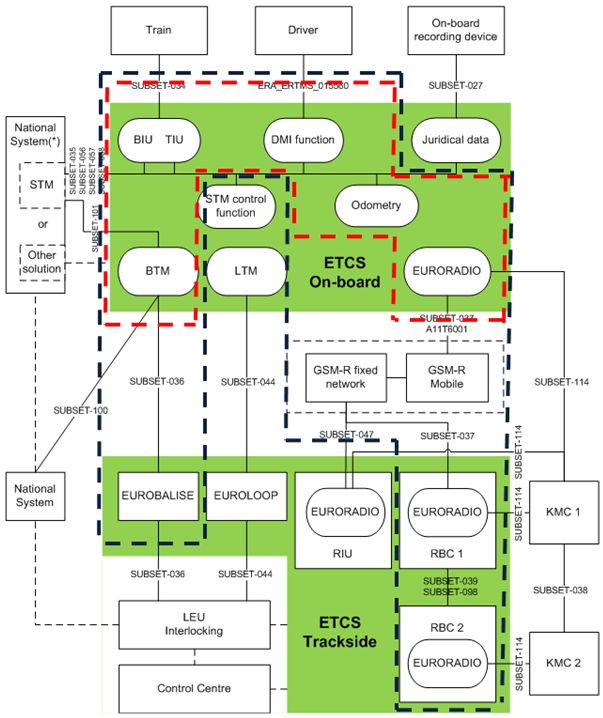
\includegraphics[width=.7\textwidth]{images/ArchitectureSRS}
\caption[Scope of openETCS OBU model system according to ERA TSI Chapter 2.5.]{Scope of openETCS OBU model system according to ERA TSI Chapter 2.5. Functional blocks in the scope of openETCS have been marked by the dashed blue line. The dashed red line shows the OBU blocks in the scope of openETCS.}
\label{f:architecture_srs}
\end{figure}


\section{Top Level Architecture and External Interfaces}
Figure~\ref{f:top_level} shows the top level architecture with external interfaces E1, E2,$\ldots$, E9.
\begin{figure}
\centering
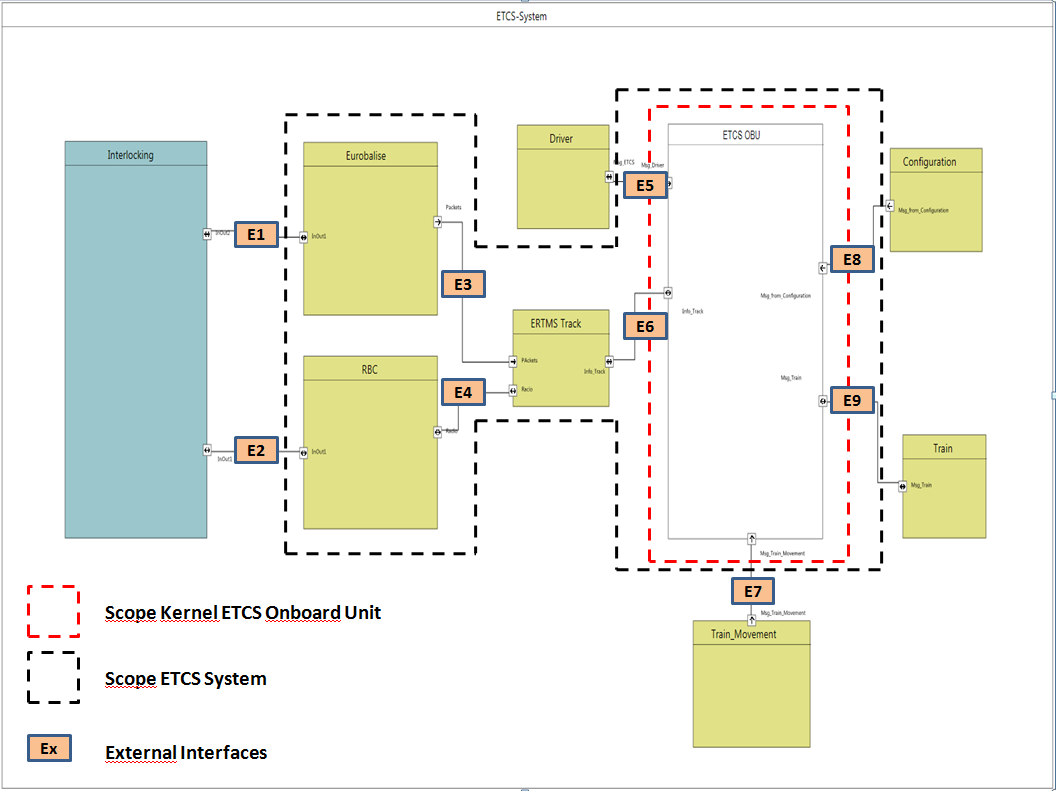
\includegraphics[width=\textwidth]{top_level_architecture.png}
\caption{Top level architecture with external interfaces.}
\label{f:top_level}
\end{figure}
The external interfaces are used for the communication between the openETCS OBU (dashed red line) and systems out of the scope of the openETCS project and the ETCS Onboard Unit System.\todo[fancyline]{paragrapoh has to be checked and extended to be more clear} In the following we give  brief overview of the interfaces:
\begin{description}
\item[E1:] In- and out flow between the Interlocking and the Eurobalise. Only relevant for controlled Eurobalises.

\item[E2:] In- and out flow between the Interlocking and Radio Block Control.
This interface ensures the states or logics directly to the Radio Block Control and the other way back from the train to the interlocking.

\item[E3:] Input flow from the Eurobalise to the Balise Transmission Module or Antenna Unit (BTM) into the ETCS OBU.

\item[E4:] In- and out flow between the Radio Block Control and the Euroradio modul into the ETCS OBU. This interface is not active in ETCS levels 0 and 1 since there is no ETCS radio interaction between track and train in these levels.

\item[E5:] This interface is used for the interaction between the driver and the display (Driver Machine Interface, DMI), c.f.~Figure \ref{DMI Interfaces}.\todo[fancyline]{check if figure is correct. Do we need this figure anyway? If so, make it more appealing.}
\begin{figure}
\centering
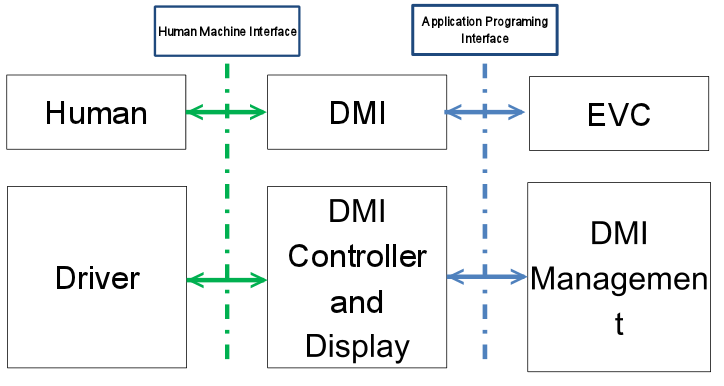
\includegraphics[scale=0.5]{images/DMIinterfaces}
\caption{DMI Interfaces.}
\label{DMI Interfaces}
\end{figure}

\item[E6:] This interface is a compound structure and combines the interfaces E3 and E4.

\item[E7:] Input interface to the odometry subsystem of the ETCS OBU. Used for sending information to the train if there is any movement outside the ETCS System, e.g.~"cold movement".

\item[E8:] Input interface to the ETCS OBU to set configuration data such as fixed values, system values, national values and train configuration.

\item[E9:] In- and Out flow between the ETCS OBU and the train. This interface is used for the interaction between the Train and the ETCS OBU such as brake control, traction control, door control, etc.
\end{description}





{\Huge !!Rest of this chapter is outdated!!}


\section{System Architecture SysML View}
The SysML System view of the architecture will reflect the scope accorgin to 4.1 and is a top down breakdown to the design layer. The functional breakdown has been done in Scade System and is part of the design model. Furthermore it will reflect all the external and internal interface that will will be described in 4.3. Another goal of the System Architecture SysML view is to explain and set the boundaries for the ETCS Kernel development "F2 Kernel" as the main design part of the openETCS@ITEA2 project.

\subsection{1st Level System Architecture View}
All subystem of the ETCS/ERTMS Basic Sytem according in the scope of the openETCS@ITEA2 project will be reflected in this 1st level view. Furthermore the interlocking as part of a full Rail Signalling System, but not part of the openETCS scope, will be highlighted in this view.

Interlocking =  interlocking is an arrangement of signal apparatus that prevents conflicting movements through an arrangement of tracks such as junctions or crossings. The signalling appliances and tracks are sometimes collectively referred to as an interlocking plant. An interlocking is designed so that it is impossible to display a signal to proceed unless the route to be used is proven safe.




\subsection{2nd Level System Architecture View}
The 2nd level system view will provide a decopmosition of the ETCS on-board unit systems and the Kernerl of the ETCS. The kernel is the main part of the ETCS Onboard Unit system and reflects the functions specified in the ERA TSI Subset 26. Therefore, the boundaries and interfaces to the other subasystems of the ETCS on-bard unit needs to be fully described and formal. At least the formalisation kernel functions and boundaries should be realized in the openETCS project.

\begin{figure}
\centering
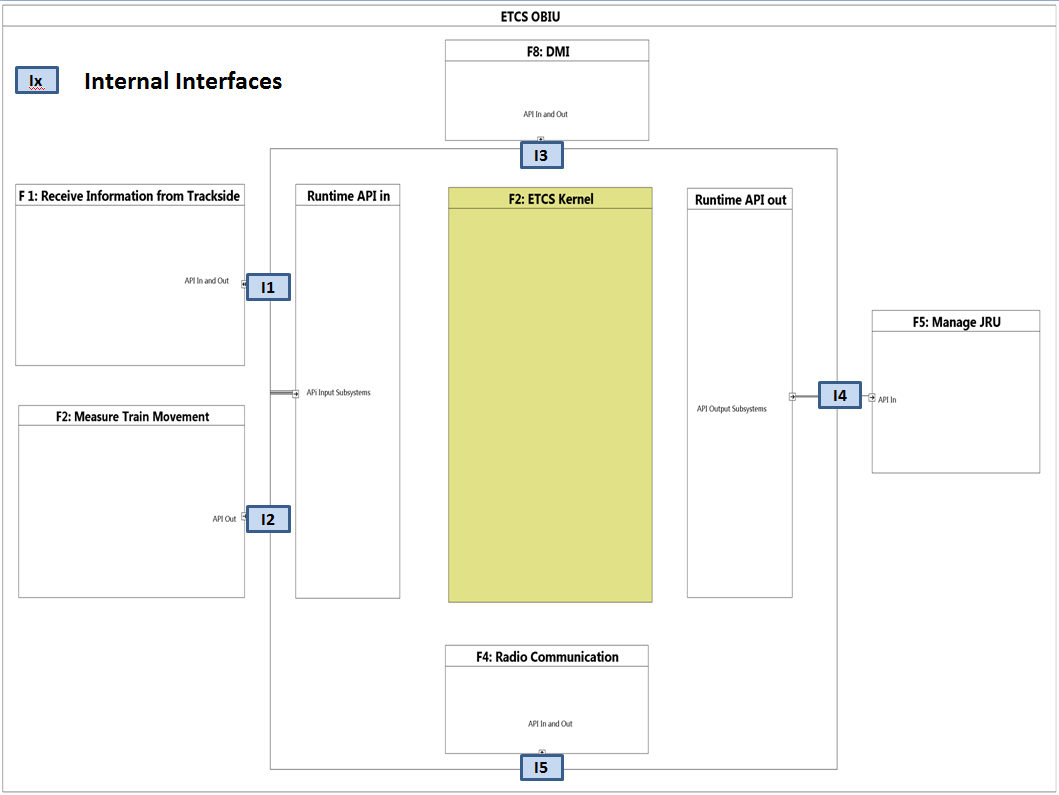
\includegraphics[width=\textwidth]{images/2ndlevelarchitecture}
\caption{2nd level system architecture view.}
\label{2nd level System Architecture view}
\end{figure}

\subsection{3rd Level System Architecture View}
The 3rd level system view will provide a decopmosition of the ETCS Kernel of the ETCS Onboard Unit Systems. The decomposition and further design of the subfunctions of the kernel are part of the chapter 6 in this document. In chapter 6 we will consider the design description that will be completed by every designer itself. The designer can decided in this layer about the decomposition and boundaries of his subsystem, but need to describe the design choices.


\section{Interfaces}
This section will consider the external and internal interfaces as described in the system decomposition figures in 4.2.1 and 4.2.2.



\subsection{Internal Interfaces}
Internal interfaces will describe the data flow between the ETCS Onboard Unit Kernel and ETCS Onboard Unit Subsystems within the ETCS Onboard Unit System.

\begin{description}
\item[I1:] In flow from the Balise Transmission Module (BTM or Antenna) to the "F2 ETCS Kernel" trough Runtime API in. Transmitted data are information from the Eurobalise.

\item[I2:] In flow from the Odometrie (ODO) to the "F2 ETCS Kernel" trough Runtime API in. Transmitted data are information from the Movement of the train.

\item[I3:] In- and Out flow between the DMI Controller and the "F2 ETCS Kernel" trough Runtime API in and out. Transmitted data are information of driver action and display. See description in figure of "External Interface E5".

\item[I4:] Out flow from "F2 ETCS Kernel" to the JRU Manager trough Runtime API out. Transmitted data are all necessary information for a juridical recorder unit "black box".

\item[I5:] In- and Out flow between the Euroradio and "F2 ETCS Kernel" trough Runtime API in and out. Transmitted data are radio track information (RBC) and information to the track (RBC). 
\end{description}

